\documentclass[11pt]{exam}

\usepackage{amssymb, amsmath, amsthm, mathrsfs, multicol, graphicx} 
\usepackage{tikz}

 \def\d{\displaystyle}
\def\?{\reflectbox{?}}
\def\b#1{\mathbf{#1}}
\def\f#1{\mathfrak #1}
\def\c#1{\mathcal #1}
\def\s#1{\mathscr #1}
\def\r#1{\mathrm{#1}}
\def\N{\mathbb N}
\def\Z{\mathbb Z}
\def\Q{\mathbb Q}
\def\R{\mathbb R}
\def\C{\mathbb C}
\def\F{\mathbb F}
\def\A{\mathbb A}
\def\X{\mathbb X}
\def\E{\mathbb E}
\def\O{\mathbb O}
\def\U{\mathcal U}
\def\pow{\mathcal P}
\def\inv{^{-1}}
\def\nrml{\triangleleft}
\def\st{:}
\def\~{\widetilde}
\def\rem{\mathcal R}
\def\sigalg{$\sigma$-algebra }
\def\Gal{\mbox{Gal}}
\def\iff{\leftrightarrow}
\def\Iff{\Leftrightarrow}
\def\land{\wedge}
\def\And{\bigwedge}
\def\AAnd{\d\bigwedge\mkern-18mu\bigwedge}
\def\Vee{\bigvee}
\def\VVee{\d\Vee\mkern-18mu\Vee}
\def\imp{\rightarrow}
\def\Imp{\Rightarrow}
\def\Fi{\Leftarrow}

%\def\={\equiv}
\def\var{\mbox{var}}
\def\mod{\mbox{Mod}}
\def\Th{\mbox{Th}}
\def\sat{\mbox{Sat}}
\def\con{\mbox{Con}}
\def\bmodels{=\joinrel\mathrel|}
\def\iffmodels{\bmodels\models}
\def\dbland{\bigwedge \!\!\bigwedge}
\def\dom{\mbox{dom}}
\def\rng{\mbox{range}}
\DeclareMathOperator{\wgt}{wgt}


\def\bar{\overline}


\newcommand{\vtx}[2]{node[fill,circle,inner sep=0pt, minimum size=4pt,label=#1:#2]{}}
\newcommand{\va}[1]{\vtx{above}{#1}}
\newcommand{\vb}[1]{\vtx{below}{#1}}
\newcommand{\vr}[1]{\vtx{right}{#1}}
\newcommand{\vl}[1]{\vtx{left}{#1}}
\renewcommand{\v}{\vtx{above}{}}

\def\circleA{(-.5,0) circle (1)}
\def\circleAlabel{(-1.5,.6) node[above]{$A$}}
\def\circleB{(.5,0) circle (1)}
\def\circleBlabel{(1.5,.6) node[above]{$B$}}
\def\circleC{(0,-1) circle (1)}
\def\circleClabel{(.5,-2) node[right]{$C$}}
\def\twosetbox{(-2,-1.4) rectangle (2,1.4)}
\def\threesetbox{(-2.5,-2.4) rectangle (2.5,1.4)}
\newcommand{\twoline}[2]{\begin{pmatrix}#1 \\ #2 \end{pmatrix}}


\def\circleA{(-.5,0) circle (1)}
\def\circleAlabel{(-1.5,.6) node[above]{$A$}}
\def\circleB{(.5,0) circle (1)}
\def\circleBlabel{(1.5,.6) node[above]{$B$}}
\def\circleC{(0,-1) circle (1)}
\def\circleClabel{(.5,-2) node[right]{$C$}}
\def\twosetbox{(-2,-1.5) rectangle (2,1.5)}
\def\threesetbox{(-2,-2.5) rectangle (2,1.5)}

%\pointname{pts}
\pointsinmargin
\marginpointname{pts}
\addpoints
\pagestyle{head}
%\printanswers

\firstpageheader{Math 228}{\bf Homework 3}{Due: Wed Feb 6, 2013}


\begin{document}
\noindent \textbf{Instructions}: Complete the homework problems below on {\em separate} sheets of paper (and not all jammed up between the questions).  This is to be turned in and graded, so make sure your work is neat and easy to ready - there is nothing wrong with using a separate sheet of paper for each problem. Each solution should be accompanied with supporting work or an explanation why the solution is correct. Your work will be graded on correctness as well as the clarity of your explanations. 

\begin{questions}
\question[8]  Consider the statement: $\forall x \forall y (x-y \ge 2 \imp \exists z (y < z \and z < x))$.
\begin{parts}
\part Explain what this statement says in words.  Is the statement true?
\begin{solution}
 The strictest translation: For all $x$ and for all $y$, if $x - y$ is at least 2, then there is a number $z$ which is larger than $y$ and less than $x$. 
 
 Alternatively, iven any two numbers $x$ and $y$, if $x$ is at least two larger than $y$, then there is a number between them.  Or even more loose: For any numbers at least two apart, there is a number between them.
\end{solution}

\part State the contrapositive of the original statement.  Do so both in words and in symbols.
\begin{solution}
 The contrapositive: for all $x$ and $y$, if there is no number $z$ larger than $y$ and smaller than $x$, then $x - y < 2$.  Or if you simplify, for all $x$ and $y$, if every $z$ is either not greater than $y$ or not less than $x$, then $x - y$ is less than $2$.
 
 \[\forall x \forall y (\forall z (y \ge z \vee z \ge x) \imp x-y < 2)\]
\end{solution}

\part State the converse of the original statement.  Is the converse true?
\begin{solution}
 The converse is, for all $x$ and for all $y$, if there is some $z$ greater than $y$ and less than $x$, then $x-y \ge 2$.  Or in symbols,
 \[\forall x \forall y (\exists z (y < z \and z < x) \imp x-y \ge 2)\]
 The converse is true, as long as we consider only the integers, but false if we consider the real numbers (or rationals).
\end{solution}

\part State the negation of the original statement.  Do so both in words and in symbols (simplifying as much as possible).
\begin{solution}
 The negation: there are numbers $x$ and $y$ such that $x - y$ is at least 2, but for all $z$, either $z$ is not larger than $y$ or not less than $x$.
 
 \[\exists x \exists y (x - y \ge 2 \and \forall z (y \ge z \vee z \ge x))\]
\end{solution}

\end{parts}

\question[6] Let $A$, $B$ and $C$ be sets.  Suppose that $A \subseteq B$ and $B \subseteq C$.  Does this mean that $A \subseteq C$?  Explain how you know (i.e., prove your answer).

\begin{solution}
 Yes it does.  We can see this using a Venn diagram - the circle $A$ is completely contained in the circle $B$, and the circle $B$ is completely contained in the circle $C$.  So the circle $A$ is completely contained in the circle $C$.  
 
 Suppose $A \subseteq B$ and $B \subseteq C$.  Then take any $x \in A$.  Since $A \subseteq B$, we have that $x \in B$ as well - that is, everything in $A$ is also in $B$, so this works for the arbitrary $x$ we chose.  Now that we know that $x \in B$, we can conclude $x \in C$, since $B \subseteq C$ - everything in $B$ is also in $C$.  Since $x$ was an arbitrary element of $A$, which we showed was also in $C$, we have $A \subseteq C$ - everything in $A$ is also in $C$.
\end{solution}


\question[6] 
\begin{parts}
  \part Draw a Venn diagram for the set $S = \bar A \cup (B \cap \bar C)$.
     \begin{solution}
	    \begin{center}
		  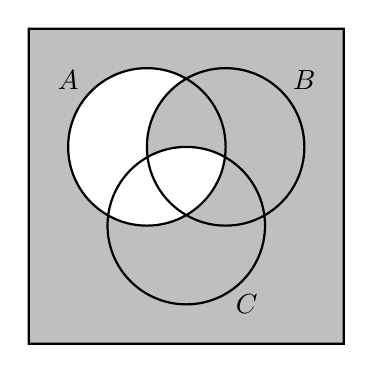
\begin{tikzpicture}[fill=gray!50]
		  \fill \threesetbox;
	    \begin{scope}
	      \clip \threesetbox \circleB;
	      \fill[white] \circleA;
	    \end{scope}
	    \begin{scope}
	      \clip \circleC;
	      \fill[white] \circleA;
	    \end{scope}

	    \draw[thick] \circleA \circleAlabel \circleB \circleBlabel \circleC \circleClabel \threesetbox;
	    \end{tikzpicture}
	    \end{center}
    \end{solution}
    
  \part For the Venn diagram given below, express the shaded set in terms of $A$, $B$, and $C$.  Simplify your answer so that bars are only directly over letters.
      \begin{center}
      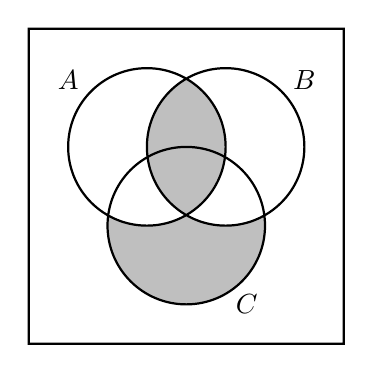
\begin{tikzpicture}[fill=gray!50]
	\fill \circleC;
	\begin{scope}
	    \clip \circleC;
	    \fill[white] \circleA \circleB;
	  \end{scope}
	\begin{scope}
	  \clip \circleA;
	  \fill \circleB;
	\end{scope}
\draw[thick] \circleA \circleAlabel \circleB \circleBlabel \circleC \circleClabel \threesetbox;
\end{tikzpicture}
\end{center}

    \begin{solution}
      The shaded region includes everything which is both in $A$ and $B$, and also the part of $C$ which is not in $A$ or $B$.  Therefore the set is \[(A \cap B) \cup (C \cap \bar{A \cup B},\] which can be simplified to
      \[(A \cap B) \cup (C \cap \bar A \cap \bar B)\]
    \end{solution}

    
\end{parts}




\uplevel{{\bf Writing Assignment:} Please turn in the following writing assignment separately from the problems above (i.e., on a separate sheet of paper, NOT stapled to the rest of the problems). }

\question[10] In class on Friday (February 1st) we discovered that a graph has an Euler circuit if and only if every vertex has even degree.  Pick either the ``if'' or ``only if'' part of the statement and explain how we know it works.  Clearly state which direction you choose to justify.

\begin{solution}
 The ``only if'' part is much easier: if a graph has an Euler circuit, then every vertex has even degree.  Suppose we have a graph that has an Euler circuit.  Consider first the vertex we start at - call it $v_0$.  The Euler circuit uses every edge exactly once, and we must end at $v_0$.  We start the circuit, leaving $v_0$ by one of the edges.  Eventually we will need to return to $v_0$, using a second edge.  Perhaps we will leave $v_0$ again, but every time we do, we know we must eventually return (since we finish the circuit by returning to $v_0$).  So for every edge which we leave $v_0$ by, there is a second edge which we return by.  Thus the edges adjacent to $v_0$ come in pairs - the leaving edges and the returning edges - so there are an even number.  That is, the degree of $v_0$ is even.
 
 Now consider any other vertex in the graph, say $v_1$.  The Euler circuit neither begins, nor ends, at $v_1$.  So every time we take an edge {\em to} $v_1$, we must also take a different edge {\em from} $v_1$.  So again, the edges adjacent to $v_1$ can be divided into two equal sets - the arriving edges and the departing edges.  Therefore the number of edges adjacent to $v_1$ is even.  This works for all vertices other than $v_0$.  
 
 If you try to justify the ``if'' part - that if every vertex of a graph has an even degree, then it has an Euler circuit - you will need to describe how to generate the Euler circuit for any such graph.  This is not easy.  The idea is this: start at any vertex and create a circuit.  That is, leave the vertex, start traveling along edges, until you arrive back at the starting vertex.  First, we must justify that you won't get stuck - this is because if you did get stuck somewhere, say at $v_1$, then $v_1$ must have had an odd degree (more incoming than outgoing edges) but we know this is false.  So you never get stuck.  However, we don't know that you use all the edges.  Never fear: if there was an edge which you did not use, then there must be an unused edge adjacent to some vertex you visited along your first guess at a circuit.  Redraw your circuit, this time when you get to that vertex with the extra edge, pause your original circuit and go on a little ``side quest'' incorporating the new edge.  You will create an circuit using only edges not used in the original circuit (we know you can do this because you will never get stuck - all the vertices in the ``side quest'' will still have even degree, not counting the edges from the original circuit).  When you return from your side quest, continue and finish your original circuit.  Now inspect the new larger circuit you have created.  Have all the edges been used?  If so, then you are done.  If not, find another side quest to ``splice'' into your current circuit.  Continue until eventually all the edges are incorporated into the circuit.  Note, this is just a rough sketch of what you do.  To completely justify this, you need to carefully describe the algorithm and then prove that it works. 
\end{solution}

\end{questions}




\end{document}


